\documentclass[11pt]{article}

\usepackage{ifthen}
\usepackage{geometry}
\usepackage[usenames,dvipsnames]{color}
\usepackage{marvosym}
\usepackage{wasysym}
\usepackage{enumitem}
\usepackage{setspace}
\usepackage{url}
\usepackage{multicol}
\usepackage{paracol}
\usepackage{fontspec}
\usepackage{xeCJK}
\usepackage{changepage}
\usepackage{listings}
\usepackage{graphicx}

\thispagestyle{empty}\pagestyle{empty}

\XeTeXlinebreaklocale "zh"
% \setCJKmainfont{Source Han Serif SC}

\input{cv.tex}

\begin{document}

\cvtitle{\textbf{杨睿妮}}{BrickRed}{}{0.5cm}

\positionedbox{left}{0.7\textwidth}{%
	邮箱:\url{yangruinii@163.com}\\
	Github:\url{https://github.com/KKKirino}
}

\begin{picture}(0, 0)
	\put(455, -10){\hbox{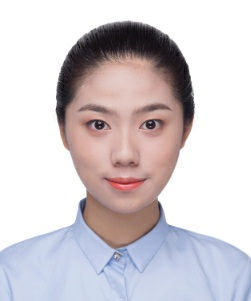
\includegraphics[scale=0.4]{./avatar.png}}}
\end{picture}

\positionedbox{right}{0.3\textwidth}{
	% \begin{picture}(50,50)
	% 	\put(480,0){\hbox{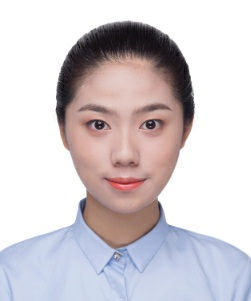
\includegraphics[scale=0.3]{./avatar.png}}}
	% \end{picture}
}

\vspace{0.7cm}

\cvsectiontitle{\textbf{教育背景}}
\cvcompany{学士,电子科技大学}{2018.09 - 至今}\\
英才实验学院(工科实验班),计算机科学专业\\

\vspace{.1cm}

GPA: 3.99 / 4.00,CET-4 成绩 601,CET-6 成绩 553 \\
\textbf{数理课程成绩:}数学分析 87、随机数学及概率论 93、线性代数 91、离散数学 98 \\
\textbf{计算机专业课成绩:}数据结构与算法 85、操作系统 91、计算机网络 87、人工智能 99

\vspace{0.8cm}

\cvsectiontitle{\textbf{项目\&研究经历}}
\vspace{-1cm}
\begin{itemize}[leftmargin=0.5cm]
	\item \cvcompany{基于强化学习的非真实感草稿渲染简化}{2020.09 - 至今}\cvsublevel{%
		\cvsubbullet{%
			通过编码器对图像降维,利用了强化学习框架,将艺术家的草稿进行简化,以生成直接用于上色的线稿。研究相关领域已有成果,参考了早稻田大学的一系列线稿简化工作,基于其结果上优化。%
		}%
		\cvsubbullet{%
			使用 Pytorch 框架基于 CartoonGAN, AdaIN 以及 U-Net 模型进行优化。
		}
	}

	\item \cvcompany{基于 Flutter 的聊天应用}{2020.12}\cvsublevel{%
		\cvsubbullet{%
			属于个人项目,尝试使用谷歌的 Flutter 跨平台应用开发框架实现类似 QQ 简洁版的界面 UI,并计划使用 Leancloud 的即时聊天 API 以及声网的音视频 API 完成完整的聊天功能。%
		}%
	}

	\item \cvcompany{人工智能课程设计}{2020.09 - 2020.11}\cvsublevel{%
		\cvsubbullet{
			\url{https://github.com/KKKirino/Coding-Every-Day/tree/master/2020/ai-course-exercise}
		}
		\cvsubbullet{%
			主要包括 A* 启发式搜索算法解决八数码问题、手动实现决策树的建立和剪枝过程、手动实现包含一个隐层和 Sigmoid 激活函数的神经网络的反向传播算法。%
		}%
		\cvsubbullet{%
			使用 Python 实现,严格遵守 PEP8 代码风格规范,使用 Python 3 Typing 系统提升代码的可阅读性,为函数提供完整的注释,保证代码质量。
		}
	}

	\item \cvcompany{暑期专业生产实习:全国航班大数据可视化平台}{2020.06 - 2020.08}\cvsublevel{%
		\cvsubbullet{%
			于大二下学期开展的暑期生产实习项目,基于 Flask + Spark 框架对全国航班数据进行爬取,并对爬取到的数据使用 Spark 框架进行分析,并保存到 MySQL 数据库中,通过前端页面进行展示。%
		}%
		\cvsubbullet{%
			负责前端页面展示部分,将数据通过 Ajax 请求加载到前端界面,并使用 ECharts 图表库进行可视化。
		}
	}
\end{itemize}

\vspace{0.4cm}
\cvsectiontitle{\textbf{荣誉\&奖项}}
\vspace{-0.8cm}
\begin{adjustwidth}{0.05cm}{0cm}
	\cvcompany{\small{Google HashCode 编程挑战赛,国际排名 \#1736(Top 15\%),中国区域排名 \#32}}{2021.02}\\%
	\cvcompany{\small{APMCM 亚太地区大学生数学建模二等奖}}{2020.11}\\%
	\cvcompany{\small{连续两年获得英才实验学院优秀奖学金二等奖}}{2019, 2020}\\%
\end{adjustwidth}
\end{document}
